\documentclass[UTF8]{ctexart}

\usepackage{geometry}
    \geometry{left=4cm,right=4cm,top=2cm,bottom=2cm}
\usepackage{amsmath}
\usepackage{amssymb}
\usepackage{caption} 	 % 标题
\usepackage{xcolor} 	 % 颜色
\usepackage{graphicx} 	 % 引用图片
\usepackage{float}
\usepackage{multirow}
\usepackage{framed} 	 % 方框 \begin{framed}

\usepackage{indentfirst} 	 % 首行缩进 
    \setlength{\parindent}{0em}
\usepackage{setspace} 	 % 行间距 \begin{spacing}{arg}

\usepackage{extarrows} 	 % 箭头宏包 \vv{}
\usepackage{esvect} 	 %向量箭头
\usepackage[version=3]{mhchem} 	 %化学方程式 \ce{}
\usepackage{siunitx} 	 %国际单位 \si{unit} \SI{number}{unit} 


% font
\newcommand{\ve}[1]{\boldsymbol{\mathbf{#1}}}
\newcommand{\unit}[1]{\boldsymbol{\mathbf{\hat{#1}}}}
\newcommand{\mcal}{\mathcal}
\newcommand{\mscr}{\mathscr}
% common symbol
\newcommand{\E}{\mathrm e}
\renewcommand{\I}{\mathrm i}
\newcommand{\R}{\mathbb R}
\newcommand{\Z}{\mathbb Z}
\newcommand{\N}{\mathbb N}
\newcommand{\Q}{\mathbb Q}
\newcommand{\C}{\mathbb C}
% differentiation
\def \DD #1.#2.#3 {\dfrac{d^{#1} #2}{d #3^{#1}}}
\def \PP #1.#2.#3 {\dfrac{\partial^{#1} #2}{\partial #3^{#1}}}
\def \dd #1.#2 {\dfrac{d #1}{d #2}}
\def \pp #1.#2 {\dfrac{\partial #1}{\partial #2}} 
\newcommand{\del}{\nabla}
% matrix
\newcommand{\transp}{^{\top}}
\DeclareMathOperator{\tr}{tr}
\newcommand{\diag}{\operatorname{diag}}


\begin{document}
\section{线性方程组}
\subsection{关键概念}
\subsubsection*{$ n $ 元线性方程} 
$ a_1 x_1 + a_2 x_2 + \cdots + a_n x_n = b $

\subsubsection*{齐次线性方程组} 
\[ \begin{cases}
a_{11} x_1 + a_{12} x_2 + \cdots + a_{1n} x_n = b_1 \\
a_{21} x_1 + a_{22} x_2 + \cdots + a_{2n} x_n = b_2 \\
\hskip 7em \vdots \\
a_{m1} x_1 + a_{m2} x_2 + \cdots + a_{mn} x_n = b_m \\
\end{cases} \]
当上面方程组中 $ b_i \ ( i = 1, 2, \dots, m ) $ 均为零时, 上述方程组为线性方程组. 反之则为非齐次线性方程组. 

\subsubsection*{解} 
线性方程组的一个解为满足该方程组的一个向量(有序数组). 
\[ (x_1, x_2, \dots, x_n) \]
若该向量为零向量则称其为零解.

\subsubsection*{主元 | 主元列 } 
阶梯形矩阵中每行的非零首元素, 如下面的红色元素
\[ 
\begin{bmatrix}
    \color{red} 3 & 2 & 9 & 4 \\
    0 & \color{red} 4 & 1 & 1 \\
    0 & 0 & \color{red} 1 & 0 \\
    0 & 0 & 0 & \color{red} 6
\end{bmatrix} 
\]
主元所在列为主元列.
\vskip 1em
在本文章中, 为了书写方便, 在不引起歧义的情况下, 常省略不写零元素. 所以上面的矩阵亦可写作:
\[ 
\begin{bmatrix}
    \color{red} 3 & 2 & 9 & 4 \\
     & \color{red} 4 & 1 & 1 \\
     &  & \color{red} 1 &  \\
     &  &  & \color{red} 6
\end{bmatrix} 
\]



\subsection{特殊矩阵}
\subsubsection*{方阵}
行数和列数相等的矩阵称为 {\bf $ n $ 阶矩阵}, 也称方阵.

\subsubsection*{阶梯形矩阵 (REF)}
\begin{framed}
    \vspace{-0.7em}
    \paragraph{定义 --- 阶梯形矩阵}
    满足下面两个条件的为阶梯形矩阵:
    \begin{itemize}
        \item 非零行在零行之上
        \item 某一行的主元在前一行元素右面
    \end{itemize}
\end{framed}

\subsubsection*{简化阶梯形矩阵 (RREF)}
\begin{framed}
    \vspace{-0.7em}
    \paragraph{定义 --- (行)简化阶梯形矩阵}
    若一个阶梯形矩阵还满足:
    \begin{itemize}
        \item 主元均为 $ 1 $
        \item 主元为该主元列中唯一的非零元素
    \end{itemize}
    则称其为简化阶梯形矩阵.
\end{framed}

\subsubsection*{对角矩阵}
行数等于列数(方阵), 且除对角线上的元素, 其余元素均为 $ 0 $. 记作: 
\[ \ve D = \diag(\lambda_1, \lambda_2, \dots, \lambda_n) \]
\[ \begin{bmatrix}
    \lambda_1   & 0           & \cdots & 0        \\
    0             & \lambda_2 & \cdots & 0        \\
    0             & 0           & \ddots & \vdots   \\
    0             & 0           & \cdots & \lambda_n 
\end{bmatrix} \]

\subsubsection*{单位矩阵}
主对角线上所有元素均为 $ 1 $ 的对角矩阵. 记作:
\[ \ve I = \diag(1, 1, \dots, 1) \]
\[ \begin{bmatrix}
    1         &        &  &         \\
             & 1       &  &         \\
             &        & \ddots &   \\
             &        &  & 1 
\end{bmatrix} \]

\subsubsection*{数量矩阵}
\[ \lambda \ve I = \diag(\lambda, \lambda, \dots, \lambda) \]

\subsubsection*{三角矩阵}
主对角线以下元素全为 $ 0 $ 的为上三角矩阵, 反之为下三角矩阵.



\subsection{行初等变换}
\paragraph{互换}
\[ \begin{bmatrix}
    \ve A_m \\
    \ve A_n
\end{bmatrix}
\sim
\begin{bmatrix}
    \ve A_n \\
    \ve A_m
\end{bmatrix} \]

\paragraph{数乘}
\[ \begin{bmatrix}
    \vdots \\
    \ve A_i \\
    \vdots 
\end{bmatrix}
    \sim
\begin{bmatrix} 
    \vdots \\
    k \cdot  \ve A_i  \\
    \vdots
\end{bmatrix} \]

\paragraph{倍加}
\[
\begin{bmatrix}
\ve A_m \\
\ve A_n
\end{bmatrix}
\sim
\begin{bmatrix}
\ve A_m + \ve A_n \\
\ve A_n
\end{bmatrix}
\]
\[
\begin{bmatrix}
\ve A_m \\
\ve A_n
\end{bmatrix}
\sim
\begin{bmatrix}
\ve A_m + k \cdot \ve A_n \\
\ve A_n
\end{bmatrix}
\]

经行初等变换得到的矩阵等价, 对于线性方程组解的情况相同. 




\subsection{方程组解的判定}
\begin{framed}
    \vspace{-0.7em}
    \paragraph{有/无解的判定}
    将增广矩阵化为阶梯形矩阵, 若其中出现 $ (b \neq 0) $
    \[ \begin{bmatrix}
        0 & 0 & \cdots & 0 & b
    \end{bmatrix} \]
    的行, 则无解. 反之有解.
\end{framed}

\begin{framed}
    \vspace{-0.7em}
    \paragraph{解的个数判定}
    满足下面等价条件即有唯一解:
    \begin{itemize}
        \item \textbf{主元个数等于变量个数} (主要)
        \item 主元列数等于系数矩阵列数 (主要)
        \item 系数矩阵与增广矩阵非零行数相同
    \end{itemize}
    反之则有无数解.
\end{framed}






\newpage
\section{矩阵代数}
\subsection{概念}
\paragraph{零矩阵}
每个元素都为零. 记作 $ \ve 0_{m \times n} $ 或 $ \ve 0 $.

\paragraph{同型矩阵}
行数和列数对应相等的矩阵, 形状相同.

\paragraph{相同矩阵}
同型, 且对应元素均相等的矩阵.





\subsection{矩阵的代数运算}
\begin{framed}
    \vspace{-0.7em}
    \paragraph{定义: 矩阵加法}
    同型矩阵相加, 等于将对应元素相加.
    \[ [a_{ij}]_{m \times n} + [b_{ij}]_{m \times n} = [a_{ij} + b_{ij}]_{m \times n} \]
\end{framed}

\begin{framed}
    \vspace{-0.7em}
    \paragraph{定义: 矩阵数乘}
    矩阵乘以一个常数, 等于矩阵的每一个元素乘以该常数.
    \[ c \cdot [a_{ij}]_{m \times n} = [c \cdot a_{ij}]_{m \times n} \]
\end{framed}

矩阵的\textbf{加法}和\textbf{数乘}统称矩阵的\textbf{线性运算}.

\vskip 1em
实数拥有的运算规则对于矩阵的线性运算仍然成立.

\begin{framed}
    \vspace{-0.7em}
    \paragraph{定义: 线性组合}
    定义矩阵 $ \ve M_1 $, $ \ve M_2 $, \dots, $ \ve M_n $ 和数 $ c_1 $, $ c_2 $, \dots, $ c_n $. 经线性运算得到的: 
    \[ \sum_{i = 1}^n c_i \ve M_i = c_1 \ve M_1 + c_2 \ve M_2 + \cdots + c_n \ve M_n \]
    称为以上矩阵的\textbf{线性组合}. 其中: $ c_1 $, $ c_2 $, \dots, $ c_n $ 称为\textbf{权}.
\end{framed}

\newpage
\begin{framed}
    \vspace{-0.7em}
    \paragraph{定义: 矩阵乘法}
    定义矩阵 $ \ve C_{m \times p} = \ve A_{m \times n} \ve B_{n \times p} $.

    \begin{center}
        $ \ve C_{ij} $ 为 $ \ve A $ 的第 $ i $ 行与 $ \ve B $ 的第 $ j $ 列对应元素相乘再相加.
    \end{center}

    把 $ \ve A $ 的第 $ i $ 行和 $ \ve B $ 的第 $ j $ 列看成向量, 则将其点乘, 所得结果即为 $ (\ve A \ve B)_{ij} $.

    用公式表示:
    \[ (\ve A \ve B)_{ij} = \sum_{k = 1}^n a_{ik} b_{kj} \]

    可见 $ \ve A $ 的列数应和 $ \ve B $ 的行数一致.
\end{framed}

图解:
\begin{figure}[H]
     \centering
     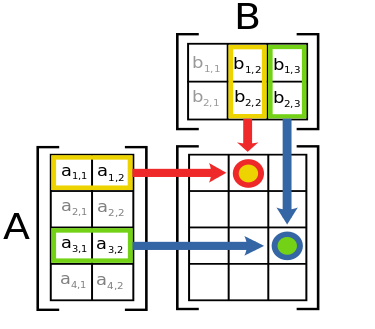
\includegraphics[width = 0.5\linewidth]{Matrix_multiplication.png}
\end{figure}

\begin{framed}
    \vspace{-0.7em}
    \paragraph{矩阵乘法的性质}
\begin{itemize}
    \item 一般不满足交换律: $ \ve A \ve B \neq \ve B \ve A $
    \item 结合律: $ (\ve A \ve B) \ve C = \ve A (\ve B \ve C) $
    \item 左分配律: $ (\ve A + \ve B) \ve C = \ve A \ve C + \ve B \ve C $
    \item 右分配律: $ \ve A (\ve B + \ve C) = \ve A \ve B + \ve A \ve C $
    \item $ \lambda(\ve A \ve B) = (\lambda \ve A) \ve B = \ve A (\lambda \ve B) $
\end{itemize}
\end{framed}

若 $ \ve{AB} = \ve{BA} $, 则称 $ \ve A $, $ \ve B $ 可交换, 典型的例子有:
\begin{itemize}
    \item 对角矩阵相乘: $ \diag(a_i) \diag(b_i) = \diag(b_i) \diag(a_i) = \diag(a_i b_i) $

    \item 与单位或数量矩阵或零矩阵相乘: $ \ve M \ve I = \ve I \ve M $, $ \ve M \ve 0 = \ve 0 \ve M = \ve 0 $

    \item 方块矩阵相乘为单位矩阵或数量矩阵: $ \ve A \ve B = \lambda \ve I \Leftrightarrow \ve B \ve A = \lambda \ve I $


\end{itemize}




\subsection{方阵的幂}
\subsubsection{单位矩阵与数量矩阵}
对角线全是 $ 1 $ 而其他位置全是 $ 0 $ 的方阵为单位方阵, $ n $ 阶单位方块矩阵记为 $ \ve I_n $. $ \lambda \ve I $ 为数量矩阵. 单位矩阵为方块矩阵的单位元, 好比数的单位元 $ 1 $; 而 $ \lambda \ve I $ 类比数字的 $ \lambda $.  
\[ 
\ve I_3 =
\begin{bmatrix}
  1 &  &  \\
   & 1 &  \\
   &  & 1
\end{bmatrix} \qquad
\lambda \ve I_3 =
\begin{bmatrix}
  \lambda &  &  \\
   & \lambda &  \\
   &  & \lambda
\end{bmatrix}
.\]

\subsubsection{性质}
\[ \ve I \ve M  = \ve M \qquad \ve M \ve I = \ve M \]

注意: $ \ve I $ 的阶数由 $ \ve M $ 决定. 更准确的写法: $ \ve I_n \ve M_{n \times p} = \ve M $.
\[ \ve I^n = \ve I \]


\subsubsection{方块矩阵的幂及性质}

\begin{framed}
    \vspace{-0.7em}
    \paragraph{定义: 方块矩阵的幂}
    设 $ \ve M $ 为 $ n $ 阶矩阵, 则有限个 $ \ve M $ 的乘积 $ \ve{MM} \cdot \ve M $ 有意义, 记作:
    \[ \ve M^k = \underset{k \text{个}}{\underbrace{\ve{MM} \cdots \ve M}} .\]
    非方块矩阵没有幂.
\end{framed}

\begin{framed}
    \vspace{-0.7em}
    \paragraph{性质}
    \[ \ve M^0 = \ve I \]
    \[ \ve M^a \ve M^b = \ve M^{a + b} \qquad \big(\ve M^a\big)^b = \ve M^{ab} \]
    \[ (\ve{AB})^n = \ve{ABAB} \cdots \ve{AB} \neq \ve A^n \ve B^n  \]
    \[ (\ve{AB})^n = \ve A (\ve{BA})^{n-1} \ve B \]
    \[ (\lambda \ve I)^n = \lambda^n \ve I \]
\end{framed}


\subsubsection{*双重求和}
单个求和符号可以看成一维的求和:
\[ \sum_{i = 1}^n a_i = a_1 + a_2 + a_3 + \cdots + a_{n - 1} + a_n  .\]

双重求和可看成二维的求和:
~
\begin{align*}
    \sum_{j = 1}^m \sum_{i = 1}^n a_i b_j =
    &a_1 b_1 + a_2 b_1 + a_3 b_1 + \cdots + a_n b_1 + \\
    &a_1 b_2 + a_2 b_2 + a_3 b_2 + \cdots + a_n b_2 + \\
    &a_1 b_3 + a_2 b_3 + a_3 b_3 + \cdots + a_n b_3 + \\
    \qquad & \vdots \\
    &a_1 b_m + a_2 b_m + a_3 b_m + \cdots + a_n b_m
\end{align*}

可以看出: \textbf{水平方向是对} $ a_i $ \textbf{的求和展开}, \textbf{竖直方向是对} $ b_j $ \textbf{的求和展开}.

图注:
\[
a_i b_j 
~~~~\Rightarrow~~~~
\underset{\xrightarrow{~~~~~~~~~~~}}{{\color{red}a_1} b_j + {\color{red}a_2} b_j + \cdots + {\color{red}a_n} b_j }
~~~~\Rightarrow~~~~  
\begin{matrix}
a_1 {\color{blue}b_1} + a_2 {\color{blue}b_1} + \cdots + a_n {\color{blue}b_1} + \\
a_1 {\color{blue}b_2} + a_2 {\color{blue}b_2} + \cdots + a_n {\color{blue}b_2} + \\
\vdots \\
a_1 {\color{blue}b_m} + a_2 {\color{blue}b_m} + \cdots + a_n {\color{blue}b_m}
\end{matrix} 
\Bigg\downarrow
\]

有限项双重求和具有如下性质:
\begin{framed}
    \vskip 0.5em
    \textbf{分配率}:
    \[ \sum_{i = 1}^m \sum_{j = 1}^n a_i b_j = \sum_{i = 1}^m a_i \sum_{j = 1}^n  b_j \]

    \textbf{可交换}: 
    \[ \sum_{i = 1}^m \sum_{j = 1}^n a_i b_j = \sum_{j = 1}^n \sum_{i = 1}^m a_i b_j \]    
\end{framed}

关于分配率的简证:
当对 $ b_j $ 求和时, $ a_i $ 视作常量, 提到求和号外: 
\[ \sum_{i = 1}^m \sum_{j = 1}^n (a_i b_j) = \sum_{i = 1}^m \left( a_i \sum_{j = 1}^n b_j \right) ,\]

括号内, $\displaystyle \sum_{j = 1}^n b_j $ 为常量, 对 $ a_i $ 求和时提出:
\[ \sum_{i = 1}^m \left( a_i \sum_{j = 1}^n b_j \right) = \sum_{j = 1}^n b_j  \sum_{i = 1}^m a_i .\]

关于可交换: 参考上面的图注, 先展开求和 $ a_i $ 后 $ b_j $, 或先展开 $ b_j $ 后 $ a_i $ 对结果无影响.


\vskip 3em
\subsection{逆矩阵}
若两实数乘积为 $ 1 $ (乘法单位元), 一个数可称另一数的乘法逆元. 类似的,
\begin{framed}
    \vspace{-0.7em}
    \paragraph{定义: 逆矩阵}
    设 $ \ve A $ 为一个 $ n $ 阶矩阵, 若存在 $ n $ 阶矩阵 $ \ve B $, 使得
    \[ \ve A \ve B = \ve B \ve A = \ve I ,\]
    则称 $ \ve A $ 可逆,  $ \ve B $ 为 $ \ve A $ 的逆矩阵, 简称逆. $ \ve A $ 的逆是唯一的, 可记为 $ \ve A^{-1} $.
    \vskip 0.5em
    类似于矩阵的幂, 只有方块矩阵才可能有逆.

    \paragraph{性质}
    \begin{itemize}
        \item $ \left( \ve A^{-1} \right)^{-1} = \ve A $ ~~~ $\displaystyle (k \ve A)^{-1} = \dfrac{1}{k} \cdot \ve A^{-1} $

        \item 若 $ \ve A $, $ \ve B $ 可逆, $ \ve A^{-1} $, $ k \ve A \ (k \neq 0)$, $ \ve A^k $ 以及 $ \ve {AB} $ 也可逆.

        \item $ (\ve A_1 \ve A_2 \cdots \ve A_{k-1} \ve A_k)^{-1} = \ve A_k^{-1} \ve A_{k-1}^{-1} \cdots \ve A_2^{-1} \ve A_1^{-1} $

        \item $ \left(\ve A^{-1}\right)^k = \left(\ve A^k \right)^{-1} = \ve A^{-k}$
    \end{itemize}
\end{framed}

\begin{framed}
    \vspace{-0.7em}
    \paragraph{定义: 初等变换}
    互换 $ \ve P(i, j) $, 倍乘 $ \ve P(i(k)) $, 倍加: 将一行(列)的常数倍加到另一行(列)上 $ \ve P(i, j(k)) $ 统称初等变换. 矩阵初等变换可施加在行或列上.
    \vskip 1em
    将单位矩阵进行一次初等得到的矩阵叫初等矩阵, 记作上面的 $ \ve P $.
    
    \paragraph{性质} \
    \begin{center}
        矩阵 $ \ve M $ 左乘初等矩阵, 等价于对 $ \ve M $ 施加该初等矩阵对应的行变换.

        矩阵 $ \ve M $ 右乘初等矩阵, 等价于对 $ \ve M $ 施加该初等矩阵对应的列变换.    
    \end{center}

    \paragraph{初等矩阵的逆矩阵} \
    \[ \ve P^{-1}(i, j) = \ve P(i, j) \]
    \[ \ve P^{-1}(i(k)) = \ve P\Big(i\Big(\dfrac{1}{k}\Big)\Big) \]
    \[ \ve P^{-1}(i, j(k)) = \ve P(i, j(-k)) \]

\end{framed}

例: $ \ve P(2, 4) \ve M_{4 \times 5} $ 等价于将 $ \ve M $ 的 $ 2 $, $ 4 $ 行交换. $ \ve M \ve P(1, 3(t)) $ 等价于将 $ \ve M $ 第 $ 3 $ 行的 $ t $ 倍加到第 $ 1 $ 行上.

\vskip 3em
\begin{framed}
    \vspace{-0.7em}
    \paragraph{初等矩阵法求逆矩阵}
    $ \ve A $ 可逆$ \Rightarrow $ $ \ve A \ve x = \ve 0 $ 只有零解($ \ve A $ 为方阵, 主元列数等于未知数个数, 主元位置一定在对角线上) $ \Rightarrow $ $ \ve A \sim \ve I $. 若 $ \ve A $ 能经有限次行初等变换得到 $ \ve I $, 即与单位矩阵等价, 则 $ \ve A $ 可逆.
    \begin{align*}
        (\ve P_k \ve P_{k-1} \cdots \ve P_1) \ve A &= \ve I \\
        (\ve P_k \ve P_{k-1} \cdots \ve P_1)^{-1}(\ve P_k \ve P_{k-1} \cdots \ve P_1) \ve A &= (\ve P_k \ve P_{k-1} \cdots \ve P_1)^{-1} \ve I \\
        \ve A &= (\ve P_k \ve P_{k-1} \cdots \ve P_1)^{-1} \\
        \ve A^{-1} &= (\ve P_k \ve P_{k-1} \cdots \ve P_1) \ve I
    \end{align*}
    
    故将 $ \ve A $ 和 $ \ve I $ 拼合为一个矩阵 $ (\ve A \mid \ve I) $, 对其做行初等变换, 当 $ \ve A $ 化为 $ \ve I $ 时, $ \ve I $ 就变为 $ \ve A^{-1} $.
    
    \[ \ve P (\ve A \mid \ve I) = (\ve P \ve A \mid \ve P \ve I) = (\ve I \mid \ve A^{-1}) \]
    \[ (\ve A \mid \ve I) \sim (\ve I \mid \ve A^{-1}) \]
\end{framed}

常见逆矩阵:
\[ 
\ve A^{-1} = \begin{bmatrix}
    a & b \\
    c & d 
\end{bmatrix}^{-1}
= 
\dfrac{1}{|\ve A|} \begin{bmatrix}
    d & -b \\
    -c & a
\end{bmatrix} 
\]
对于三阶矩阵 $ \ve A_{3 \times 3} $ ($ \ve C_{ij} $ 为代数余子式):
\[ 
\ve A^{-1} =  \dfrac{1}{|\ve A|} \begin{bmatrix}
    \ve C_{11}& -\ve C_{12}& \ve C_{13}\\
    -\ve C_{21}& \ve C_{22}& -\ve C_{23}\\
    \ve C_{31}& -\ve C_{32}& \ve C_{33}
\end{bmatrix} \transp =
\dfrac{1}{|\ve A|} \begin{bmatrix}
    \ve C_{11}& -\ve C_{21} & \ve C_{31}\\
    -\ve C_{12}& \ve C_{22}& -\ve C_{32} \\
    \ve C_{13} & -\ve C_{23} & \ve C_{33}
\end{bmatrix}
\]


\section{特殊(方块)矩阵}
\subsection{对角矩阵}
对角矩阵具有特殊性, 计算较简单:
\[ \diag(a_i) \pm \diag(b_i) = \diag(a_i \pm b_i) \]
\[ \diag(a_i) \cdot \diag(b_i) = \diag(a_i b_i) \]
\[ \diag^n(a_i) = \diag(a_i^n) \]
\[ \diag^{-1}(a_i) = \diag(a_i^{-1}) \]
单位矩阵和数量矩阵为特殊的对角矩阵.

\vskip 4em
对角矩阵与其它矩阵相乘, 就是将对角矩阵主对角线上的元素, 依次乘到另一矩阵的对应行上 (推广见广义排列矩阵). 举例: 
\[ 
\begin{bmatrix}
    \lambda & 0 & 0 \\
    0 & \mu & 0 \\
    0 & 0 & \phi
\end{bmatrix}
\begin{bmatrix}
    a & b & c & d \\
    e & f & g & h \\
    i & j & k & l
\end{bmatrix} =
\begin{bmatrix}
    \lambda a & \lambda b & \lambda c & \lambda d \\
    \mu e & \mu f & \mu g & \mu h \\
    \phi i & \phi j & \phi k & \phi l
\end{bmatrix}
\]



\subsection{严格三角矩阵}
若一个三角矩阵的主对角线上元素全为零, 则称其为严格三角矩阵. 严格三角矩阵为幂零矩阵. 
\[ \ve U = 
\begin{bmatrix}
    0 & a & b & c \\
     & 0 & d & e \\
     &  & 0 & f \\
     &  &  & 0
\end{bmatrix}    
\]

如上, 主对角线右上方的一条线($ a $, $ d $, $ f $ 所在的线)为超对角线.


\subsection{幂零矩阵}
对于一矩阵 $ \ve M $, 若能满足: \[ \ve M^k = \ve 0 \]
即为幂零矩阵. 举例:
\[ 
\ve U = \begin{bmatrix}
    0 & {\color{red}1} & 2 & 3 \\
    0 & 0 & {\color{red}4} & 5 \\
    0 & 0 & 0 & {\color{red}6} \\
    0 & 0 & 0 & 0
\end{bmatrix}
\ve U^2 =
\begin{bmatrix}
    0 & 0 & {\color{red}4} & 17 \\
    0 & 0 & 0 & {\color{red}24} \\
    0 & 0 & 0 & 0 \\
    0 & 0 & 0 & 0
\end{bmatrix}
\ve U^3 = 
\begin{bmatrix}
    0 & 0 & 0 & {\color{red}24} \\
    0 & 0 & 0 & 0 \\
    0 & 0 & 0 & 0 \\
    0 & 0 & 0 & 0
\end{bmatrix}
\ve U^4 = 
\begin{bmatrix}
    0 & 0 & 0 & 0 \\
    0 & 0 & 0 & 0 \\
    0 & 0 & 0 & 0 \\
    0 & 0 & 0 & 0
\end{bmatrix}
\]

随着次数增大, 超对角线不断向右上角移动, 直到完全消失, 得到零矩阵. 严格下三角矩阵同理.
\[
\begin{bmatrix}
0&a&0&0&0&0&0\\ 
0&0&b&0&0&0&0\\ 
0&0&0&c&0&0&0\\ 
0&0&0&0&d&0&0\\ 
0&0&0&0&0&e&0\\ 
0&0&0&0&0&0&f\\ 
0&0&0&0&0&0&0\end{bmatrix}^{\! 4}
=
\begin{bmatrix}
0&0&0&0&abcd&0&0\\ 
0&0&0&0&0&bcde&0\\ 
0&0&0&0&0&0&cdef\\ 
0&0&0&0&0&0&0\\ 
0&0&0&0&0&0&0\\ 
0&0&0&0&0&0&0\\ 
0&0&0&0&0&0&0\end{bmatrix}
\]

注意上面的答案是怎么来的, $ abcd $: 从这个位置, 向左向下作水平和竖直的线, 交超对角线于两个元素 $ a $, $ d $, 将这两个元素及其之间的元素乘起来, 得到 $ 4 $ 次方后该位置的元素. 所以经 $ 6 $ 次方后, 仅右上角有唯一非零元素 $ abcdef $, 经 $ 7 $ 次方后, 称为零矩阵. 
\vskip 1em
像上面第一条超对角线外全为 $ 0 $ 的 $ n $ 阶矩阵, 其 $ n $ 次方为零矩阵.

\subsection{广义排列矩阵(Generalized Permutation Matrix)}
每行(列)有且仅有一个 $ 1 $ (非零元素)的方阵为排列矩阵(广义排列矩阵). 一个矩阵左乘排列矩阵, 就是将该矩阵的行重新排列. 若是广义排列矩阵, 还要乘以一个系数. 类似的, 一个矩阵右乘排列矩阵, 就是将该矩阵的列重新排列.
\[ 
\begin{bmatrix}
    0&0&1&0 \\
    1&0&0&0 \\
    0&1&0&0 \\
    0&0&0&1 
\end{bmatrix}
\begin{bmatrix}
    A_1 & A_2 \\
    B_1 & B_2 \\
    C_1 & C_2 \\
    D_1 & D_2
\end{bmatrix} =
\begin{bmatrix}
    C_1 & C_2 \\
    A_1 & A_2 \\
    B_1 & B_2 \\
    D_1 & D_2 
\end{bmatrix}
\]
\[ 
\begin{bmatrix}
    A_1&B_1&C_1&D_1\\ 
    A_2&B_2&C_2&D_2
\end{bmatrix}
\begin{bmatrix}
    0&1&0&0\\ 
    0&0&1&0\\ 
    1&0&0&0\\ 
    0&0&0&1
\end{bmatrix}
=
\begin{bmatrix}
    C_1&A_1&B_1&D_1\\ 
    C_2&A_2&B_2&D_2
\end{bmatrix}
\]

\paragraph{广义排列矩阵的逆} 
为对该矩阵中所有非零元素取逆, 再将所得矩阵转置. 记 $ (g_{ij})_{n \times n} $ 为广义排列矩阵, 于是:
\[ (g_{ij})_{n \times n}^{-1} = \left(g_{ij}^{-1}\right)_{n \times n} \transp \]


\subsection{方块矩阵的迹}
方块矩阵 $ \ve M $ 的主对角线元素之和称为它的迹, 记作 $ \operatorname{tr} M $. 方阵的迹具有如下性质:
\vskip 1em
对 $ \ve A_{m \times n} $ 和 $ \ve B_{n \times m} $, 尽管矩阵的乘法不满足交换律, 方阵相乘时交换顺序会导致乘积变化,但乘积的迹不会变, 故有:
\[ \operatorname{tr} (\ve A \ve B) = \operatorname{tr} (\ve B \ve A) \]

转置后, 迹不变:
\[ \operatorname{tr} (\ve M) = \operatorname{tr} (\ve M \transp) \]


\vskip 5em
\section{矩阵转置}
\begin{framed}
    \vspace{-0.7em} 
    \paragraph{定义: 转置}
    把矩阵 $ \ve M $ 的行写成列, 或者说把列写作行, 得到新的矩阵:
    \[ (a_{ij})_{m \times n} \Rightarrow (a_{ji})_{n \times m} \]
    该过程称为转置, 得到的新矩阵记为 $ \ve M \transp $.

    \paragraph{性质}
    \begin{itemize}
        \item $ \left( \ve M \transp \right) \transp = \ve M $
        
        \item $ (\ve A \pm \ve B) \transp = \ve A \transp \pm \ve B \transp $

        \item $ (c \ve M) \transp = c \ve M \transp $

        \item $ (\ve M_1 \ve M_2 \cdots \ve M_k) \transp = \ve M_k \transp \ve M_{k - 1} \transp \cdots \ve M_1 \transp $
    \end{itemize}
\end{framed}



\section{分块矩阵}
方块矩阵加法: 原矩阵尺寸一致, 分块尺寸一致.

分块矩阵乘法: $ \ve A \ve B $ 需满足 $ \ve A $ 列的分法和 $ \ve B $ 行的分法一样.







\end{document}